\documentclass[12pt]{report}
\usepackage[margin=1in]{geometry}
\usepackage{hyperref}
\usepackage{url}
\usepackage{xurl}
\hypersetup{breaklinks=true}
\usepackage{graphicx}
\usepackage{amsmath}
\usepackage{enumitem}
\usepackage{float}

\title{Week 10 Report}
\author{Dhanush Balusa}
\date{July 25th, 2025}

\begin{document}

\maketitle

\chapter*{Research}

\noindent \textbf{Orbit Covariance:}
\begin{enumerate}

  \item Adapting Covariance Propagation to Account for the Presence of Modeled and Unmodeled Maneuvers: \url{https://ntrs.nasa.gov/api/citations/20070018023/downloads/20070018023.pdf}

  \begin{itemize}
    \item Monte Carlo "Prop–Burn–Prop" truth model gives something solid to compare simpler, faster methods against, so they can choose the best approach for orbit prediction and risk analysis.
    \begin{itemize}
      \item Prop: Generate many slightly different satellite states (position \& velocity) using a known initial covariance to represent real-world estimation errors.
      \item Burn: Propagate each orbit to the maneuver point, apply a slightly different delta-V (to mimic execution error), then propagate forward again.
      \item Prop: Use the final positions and velocities of all the satellites to calculate the "true" covariance, showing how much uncertainty actually grows because of the imperfect maneuver.
    \end{itemize}
    \item  The paper calls Monte Carlo the "truth model" because it conveys that it is the best available approximation of reality.
    \item Three methods that were tested:
    \begin{itemize}
      \item Method A (burn, no Q): Models the maneuver exactly but ignores any uncertainty. This gives bad results if the maneuver isn’t perfect.
      \item Method B (no burn, Q): Doesn’t model the maneuver but adds uncertainty as noise. Gives better uncertainty but the orbit prediction is off.
      \item Method C (burn, Q): Models the maneuver and adds some noise to account for execution errors. Matches both the predicted orbit and the uncertainty well.
    \end{itemize}
    \item Q refers to the process noise matrix — it accounts for uncertainties like maneuver execution errors, modeling imperfections, or unmodeled forces.
    \item Good covariance estimates are critical for tasks like collision avoidance or tracking satellites after maneuvers.
    \item The test used basic physics (no atmospheric drag, etc.), but the idea works with more complex models too.
  \end{itemize}

  \item Estimation Strategies for Orbit Determination of Applications Satellites: \url{https://ntrs.nasa.gov/api/citations/19740011388/downloads/19740011388.pdf}

  \begin{itemize}
    \item Covariance matrix was used to evaluate how errors in initial conditions, tracking data, and force models (e.g. gravity) influence orbit accuracy.
    \item For satellites like GEOS-C, which operate in long-arc missions (~7 days), uncertainties in the Earth’s gravity field model are more significant than measurement noise from ground stations.
    \item The analysis reveals the radial direction is the most sensitive to geopotential errors, while cross-track and along-track components are less affected.
    \item Covariance analysis can be easily added to existing orbit determination software using stored normal and state transition matrices, enabling quick computation of error growth and parameter sensitivity.
    \item Once matrices are saved, many estimation strategies can be tested efficiently, making it a low-cost way to optimize orbit determination accuracy. However, an analyical solution is a very complex process.
  \end{itemize}

  \begin{figure}[H]
      \centering
      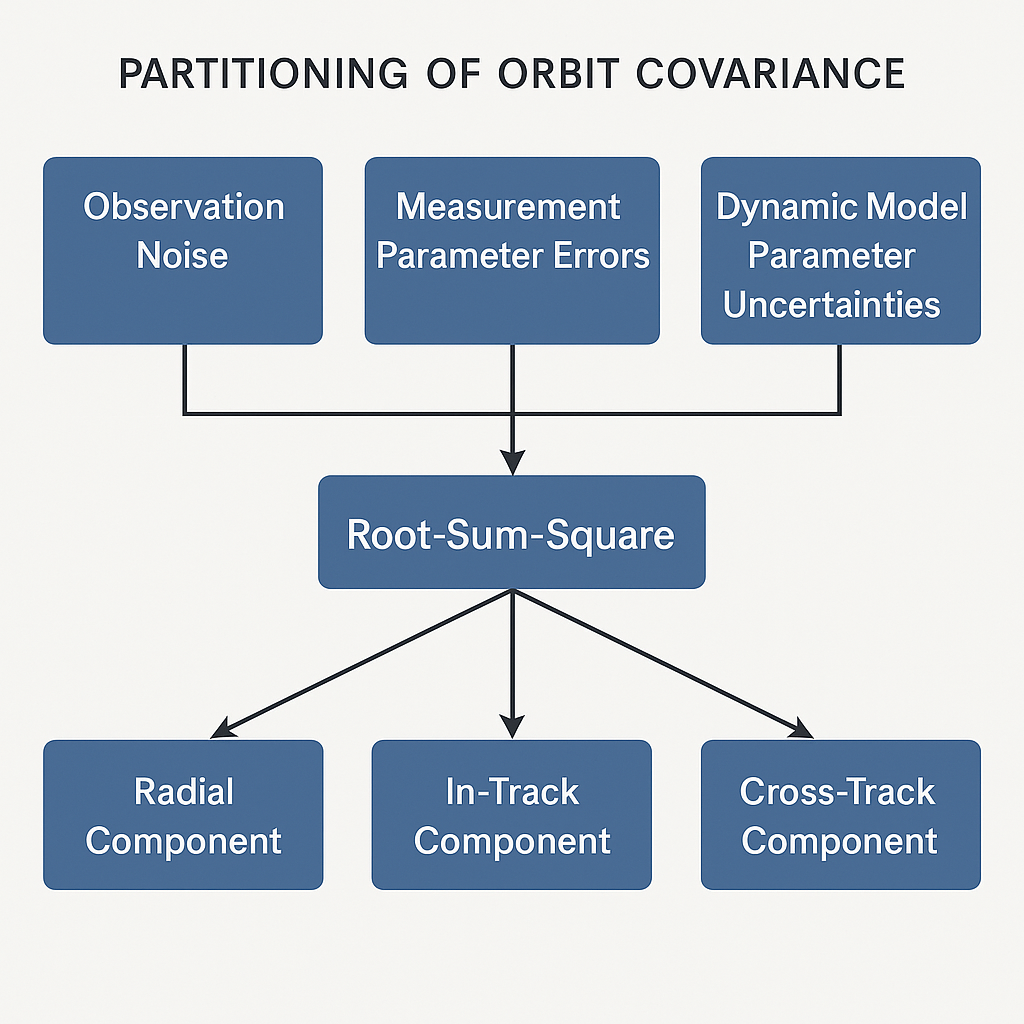
\includegraphics[width=0.8\textwidth]{figure_week_10_covariance.png}
      \caption{Simplified ChatGPT generated diagram to explain the breakdown of different types of covariance and how it's generated.}
      \label{fig:Covariance_Diagaram}
  \end{figure}

  Extra resources of analytical covariance:
  \begin{itemize}
    \item Informing Spacecraft Maneuver Decisions to Reduce Probability Informing Spacecraft Maneuver Decisions to Reduce Probability of Collision: \url{https://scholar.afit.edu/cgi/viewcontent.cgi?params=/context/etd/article/1742}
    \item A Method for Calculating Collision Probability Between Space Objects: \url{https://arxiv.org/pdf/1311.7216}
  \end{itemize}

\end{enumerate}

\noindent \textbf{How can I propogate covariance?}
  \begin{itemize}
    \item Instead of analytic integration (very complicated), using Monte Carlo is the best way.
    \item Monte Carlo modeling can be used to sample position errors from covariances and count fraction of samples that fall within the collision volume.
    \item Skyfield doesn’t support custom forces or high-precision integration — limiting my ability to account for uncertainties.
    \item Skyfield's EarthSatellite class works only from TLEs and uses the SGP4 model. Can’t directly propagate from arbitrary position-velocity states using EarthSatellite.
    \item Tools that might be able to do the job:
    \begin{itemize}
      \item OREKIT (Java or Python wrapper): supports state vector propagation and covariance. Sampling and statistical analysis aspects would be handled using standard Python libraries like NumPy and SciPy. The \texttt{PropagatorsParallelizer} can also be leveraged to efficiently run multiple propagations in parallel. 
      \item Poliastro (Python): allows propagation from state vectors, and can integrate a Monte Carlo loop easily (random sampling and statistical analysis are handled by other Python libraries like NumPy, Matplotlib, or Plotly).
    \end{itemize}
  \end{itemize}

\noindent \textbf{How to identify collision when there is covariance information?}
  \begin{enumerate}
    \item Monte Carlo Method for Collision Probability Calculations using 3D Satellite Models: \url{https://amostech.com/TechnicalPapers/2010/Integrating_Diverse_Data/deVries.pdf}
      \begin{itemize}
        \item Uses full 6x6 covariance (position \& velocity) for each object to sample many possible states using Gaussian noise.
        \item Propogates each sample pair to closest approach and checks if any are within the combined collision volume.
        \item The fraction of samples that collide gives the PoC (Probability of Collision).
        \item Uses 3D models to map important locaations on the satellite (e.g. solar panels, antennas) to determine collision volume.
        \item Monte Carlo gives statistical spread, not a single answer, so it can should the likelihood of collision.
      \end{itemize}
  \end{enumerate}

\chapter*{Code Changes}

I attempted to debug \texttt{week6-7\_fetch\_tle\_data.py} to ensure it correctly fetches the TLE sets. Nothing is still working so I will email CelesTrak for help, because the testing API may be different. If all else fails, I will see if they can give access to the main server again.
\newline \newline
After some troubleshooting with the new functions and file directory and path the \texttt{week6-7\_analyze\_approach.py} code is calculating distance, velocity, amd plotting just fine from a file with TLEs that I manually added.

\begin{figure}[H]
      \centering
      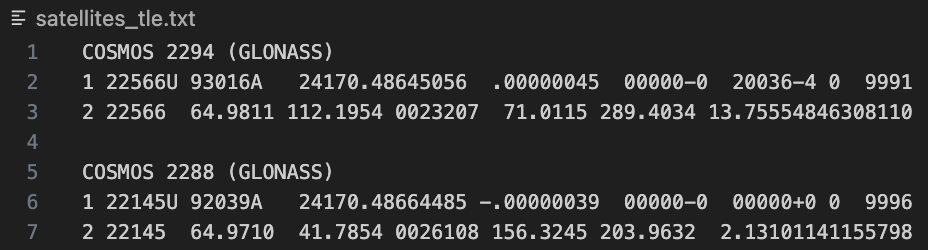
\includegraphics[width=0.8\textwidth]{figure_week_10_satellitestxt.png}
      \caption{Example of the TLE file I used to test the code.}
      \label{fig:satellitestxt}
\end{figure}

\begin{figure}[H]
      \centering
      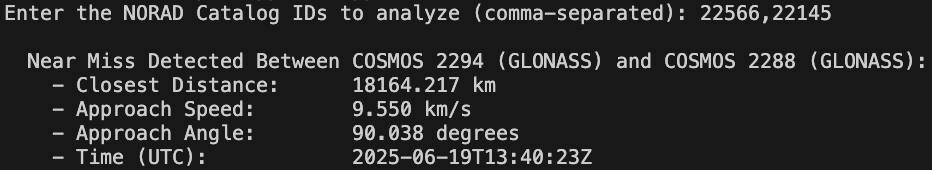
\includegraphics[width=0.8\textwidth]{figure_week_10_output.png}
      \caption{Example of the output from the code.}
      \label{fig:output}
\end{figure}

\begin{figure}[H]
      \centering
      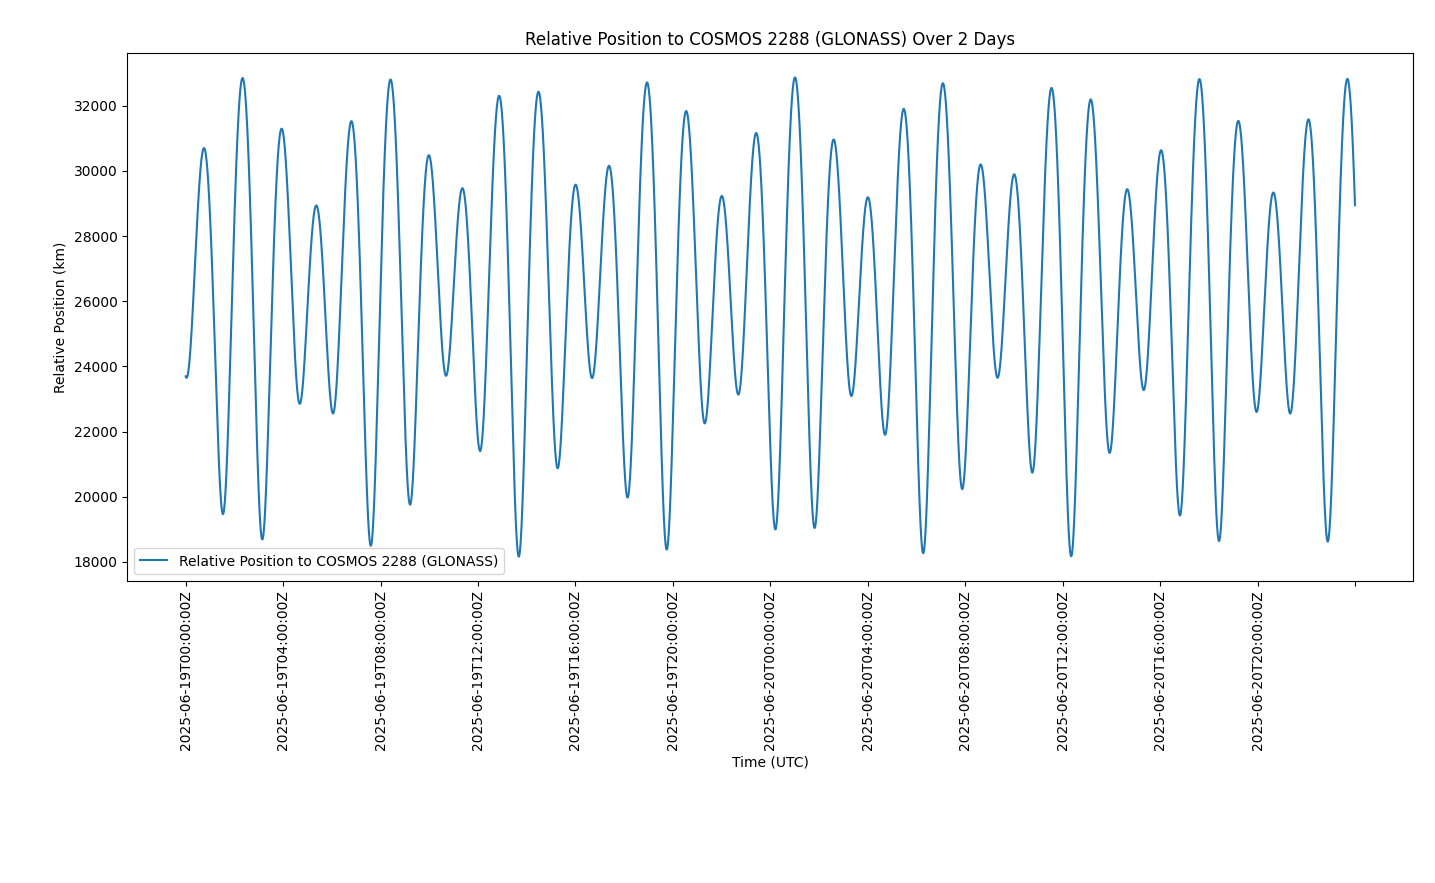
\includegraphics[width=0.8\textwidth]{figure_week_10_graph.png}
      \caption{Example of the graph generated by the code.}
      \label{fig:graph}
\end{figure}

\chapter*{Next Steps}

\textbf{My Next Steps:}
\begin{itemize}
  \item Fix the TLE fetching code and properly write them into a file.
  \item Remove the Skyfield dependency from the code and use OREKIT or Poliastro to propagate the TLEs. It will allow me to use covariance and propagate the TLEs from position-velocity states.
\end{itemize}

\noindent \textbf{Dr. Fan's feedback for next steps:}
\begin{enumerate}
  \item Flowchart of operations (of the code) to better help understand the process.
  \item Propose way(s) to fetch TLEs: by class/nature of objects? or by interest or orgin? Time: Jan-1-2025.
  \item Find some literature on TLE classes/categories, or how others are fetching TLEs for PoC purposes.
  \item TLE Propagation: Also find literature to see how to sample states/TLEs, Gaussian/Random mean and covariance.
  \item Propagate IC with initial covariance, for example space objects, and make plots.
  \item Start putting together all you have done for the final report.
\end{enumerate}

\noindent \textbf{End goals:}
\begin{itemize}
  \item Loop through all the TLEs in the different categories and calculate the approach conditions for each satellite if it is within a certain distance (e.g. 100 km) of the ISS.
  \item Incorporate covariance into space object propagation for more realistic collision identification. Also for warning time first propogate for 7 days. 
  \item Make my code a usable function so Catherine can just call it. Some input \textrightarrow{} Output (approach speed and angle).
\end{itemize}

\end{document}